\documentclass[t,xcolor=pdftex,dvipsnames,table]{beamer}
\usepackage[]{graphicx}\usepackage[]{color}
%% maxwidth is the original width if it is less than linewidth
%% otherwise use linewidth (to make sure the graphics do not exceed the margin)
\makeatletter
\def\maxwidth{ %
  \ifdim\Gin@nat@width>\linewidth
    \linewidth
  \else
    \Gin@nat@width
  \fi
}
\makeatother

\definecolor{fgcolor}{rgb}{0.345, 0.345, 0.345}
\newcommand{\hlnum}[1]{\textcolor[rgb]{0.686,0.059,0.569}{#1}}%
\newcommand{\hlstr}[1]{\textcolor[rgb]{0.192,0.494,0.8}{#1}}%
\newcommand{\hlcom}[1]{\textcolor[rgb]{0.678,0.584,0.686}{\textit{#1}}}%
\newcommand{\hlopt}[1]{\textcolor[rgb]{0,0,0}{#1}}%
\newcommand{\hlstd}[1]{\textcolor[rgb]{0.345,0.345,0.345}{#1}}%
\newcommand{\hlkwa}[1]{\textcolor[rgb]{0.161,0.373,0.58}{\textbf{#1}}}%
\newcommand{\hlkwb}[1]{\textcolor[rgb]{0.69,0.353,0.396}{#1}}%
\newcommand{\hlkwc}[1]{\textcolor[rgb]{0.333,0.667,0.333}{#1}}%
\newcommand{\hlkwd}[1]{\textcolor[rgb]{0.737,0.353,0.396}{\textbf{#1}}}%
\let\hlipl\hlkwb

\usepackage{framed}
\makeatletter
\newenvironment{kframe}{%
 \def\at@end@of@kframe{}%
 \ifinner\ifhmode%
  \def\at@end@of@kframe{\end{minipage}}%
  \begin{minipage}{\columnwidth}%
 \fi\fi%
 \def\FrameCommand##1{\hskip\@totalleftmargin \hskip-\fboxsep
 \colorbox{shadecolor}{##1}\hskip-\fboxsep
     % There is no \\@totalrightmargin, so:
     \hskip-\linewidth \hskip-\@totalleftmargin \hskip\columnwidth}%
 \MakeFramed {\advance\hsize-\width
   \@totalleftmargin\z@ \linewidth\hsize
   \@setminipage}}%
 {\par\unskip\endMakeFramed%
 \at@end@of@kframe}
\makeatother

\definecolor{shadecolor}{rgb}{.97, .97, .97}
\definecolor{messagecolor}{rgb}{0, 0, 0}
\definecolor{warningcolor}{rgb}{1, 0, 1}
\definecolor{errorcolor}{rgb}{1, 0, 0}
\newenvironment{knitrout}{}{} % an empty environment to be redefined in TeX

\usepackage{alltt}
\newcommand{\SweaveOpts}[1]{}  % do not interfere with LaTeX
\newcommand{\SweaveInput}[1]{} % because they are not real TeX commands
\newcommand{\Sexpr}[1]{}       % will only be parsed by R


%\documentclass[handout,t,xcolor=pdftex,dvipsnames,table]{beamer}  % For handout
\mode<presentation>{
\useoutertheme[subsection=false]{miniframes}
%\beamertemplatenavigationsymbolsempty
\usecolortheme{custom}
\usefonttheme[onlymath]{serif}
\setbeamercovered{invisible}
%\setbeamertemplate{navigation symbols}{}
%\setbeamertemplate{mini frames}{}  % Old one
% Comment out this line to give the header
% \setbeamertemplate{headline}[default]
\setbeamertemplate{caption}[numbered]
%\setbeamertemplate{itemize items}[circle] 
\setbeamertemplate{frametitle continuation}{\frametitle{\color{white}Title}}  % So no tile on subsequent frames, from [allowframebreaks]

%%% CUSTOMISING NAVIATION %%%%
%This customises the navigation to be thin width and just have section headings (not subsections). 
\setbeamertemplate{headline}{%
\leavevmode%
  \hbox{%
    \begin{beamercolorbox}[wd=\paperwidth,ht=2.5ex,dp=1.125ex]{palette tertiary}%   % Tertiary colour is blue
    \insertsectionnavigationhorizontal{\paperwidth}{}{\hskip0pt plus1filll}
    \end{beamercolorbox}%
}}}

\RequirePackage{marvosym}

%%% INCLUDING SOLUTIONS %%%%
%% You can incorporate both questions and solutions in the 
%% same document.  Solutions can be included between the 
%% commands \begin{soln} and \end{soln}
%% To generate a pdf with only the questions uncomment:
%\excludecomment{soln}
\usepackage{comment}
\specialcomment{soln}{\begingroup \vspace{1mm} \sl}{ \leavevmode \endgroup}

%%%% DETAILS FOR PART 1 TITLE PAGE (OLD) %%%%
%\title{\large Part2 - Probability \& Distribution Theory} 
%\subtitle{} 
%\author{\copyright Dr Di Warren 2016} 
%\date{MATH1005 - Statistics}
% \colorlet{Faculty}{Arts}
%\colorlet{Faculty}{MasterBrandRed} % This is only needed if the notes are used for different faculties.
%\colorlet{FacultyText}{White}
% Defines the color of the text used on the title page and ``blocks''
% White for Business; TitlePageBlack for Arts, Pharmacy and Science
%\definecolor{CoolBlack}{rgb}{0.0, 0.18, 0.39}

%%%% DETAILS FOR FULL COURSE TITLE PAGE %%%%
\title{\Huge STATISTICS} 
\subtitle{} 
\author{\copyright University of Sydney 2017 (Di Warren)} 
\date{MATH1005}
% \colorlet{Faculty}{Arts}
\colorlet{Faculty}{MasterBrandRed} % This is only needed if the notes are used for different faculties.
\colorlet{FacultyText}{White}
% Defines the color of the text used on the title page and ``blocks''
% White for Business; TitlePageBlack for Arts, Pharmacy and Science
\definecolor{CoolBlack}{rgb}{0.0, 0.18, 0.39}

%%%% PACKAGES %%%%
\usepackage{multirow}
\usepackage{fancybox}
\usepackage[english]{babel}
\usepackage[utf8]{inputenc}
\usepackage{bm}
\usepackage{array}
\usepackage{booktabs}
\usepackage{tikz}
\usetikzlibrary{matrix,arrows,decorations.pathmorphing}
\usepackage{verbatim}
\usepackage{pgf,pgfsys,pgffor}
\usepackage{pgfplots}
\pgfplotsset{compat=1.3} %Recommended as of Pgfplots 1.3 - necessary?
\usetikzlibrary{decorations.pathreplacing,calc}
\usetikzlibrary{shapes, backgrounds}   % For Venn diagrams
\def \setA{ (0,0) circle (1cm) }
\def \setB{ (1.5,0) circle (1cm) }
\def \setC{ (0.6,1.5) circle (1cm) }
\def \setO{ (-2, -1.5) rectangle (3.5, 2.75) }
\tikzstyle{every picture}+=[remember picture]
\tikzstyle{na} = [baseline=-.5ex]
\usepackage{listings}  %Added by Di for adding R code

%\AtBeginSection[]
%{
%   \begin{frame}
 %      \frametitle{Outline}
 %      \tableofcontents[currentsection]
%   \end{frame}
%}  %This seems overkill for weekly lecture slides.

%\AtBeginSection[]
%{
%  \begin{frame}
% \frametitle{Contents}
%  \tiny{\tableofcontents[currentsection]}
%  \end{frame}
%}
%\useoutertheme{infolines} % Just lists current section in navigation at top, nice but limiting?

%%%% TITLE PAGE AND CONTENTS AT BEGINNING OF EACH TOPIC %%%%

\RequirePackage{ifthen} % package required
\newboolean{sectiontoc}
\setboolean{sectiontoc}{true} %default to true

\AtBeginSection[]
{
\begin{frame}[plain]
\vspace{60pt}
\begin{center}
\Huge{{\textcolor{MasterBrandBlue} \insertsection}}
\end{center}
\begin{tikzpicture}[scale=0.54]
%\hspace{-12pt}
%% Big Rectangle
\fill[MasterBrandRed] (0,14) -- (20,14) -- (20,15) -- (0,15);

%\draw (1,14.5) node [anchor = west] {\textcolor{MasterBrandBlue}{\Huge{\insertsection}}}; Overlays box with title, but long titles drop off the page
\end{tikzpicture} 
\end{frame}

%%%%%WORKING VERSION OF TOC%%%%%
%\begin{frame}
%   \frametitle{Outline}
%  \tableofcontents[currentsection, sectionstyle=show/hide, subsectionstyle=show/show/hide]
%  \end{frame}
%}

%%%%%2 VERSIONS - WITH AND WITHOUT TOC%%%%%
  \ifthenelse{\boolean{sectiontoc}}{
    \begin{frame}
  \frametitle{Outline}
  \tableofcontents[currentsection, sectionstyle=show/hide, subsectionstyle=show/show/hide]
 \end{frame}
  }
}
%%%%%This doesnt seem to work?%%%%
\newcommand{\toclesssection}[1]{
  \setboolean{sectiontoc}{false}
  %\section{#1}
  \setboolean{sectiontoc}{true}
}


% PDF settings
%\hypersetup{%
%  pdftitle={\inserttitle \insertsubtitle},%
%  pdfauthor={Di Warren},%
%	pdfsubject={},%
%	pdfkeywords={}%   
%	 }

%%%%  HELPFUL MACROS %%%%
\newcommand{\ud}{\mathrm{d}}
\newcommand{\var}{\mathrm{var}}
\newcommand{\ep}{\varepsilon}
\newcommand{\cov}{\mathrm{cov}}
\newcommand{\tr}{\mathrm{tr}}
\newcommand{\MSE}{\mathrm{MSE}}
\newcommand{\rank}{\mathrm{rank}}
\newcommand{\Bias}{\mathrm{Bias}}
\newcommand{\dei}{\partial}
\newcommand{\E}{\mathbb{E}}
\newcommand{\N}{\mathcal{N}}
\newcommand{\bbR}{\mathbb{R}}
\newcommand{\V}{\mathbb{V}}
\newcommand{\betahat}{\hat{\beta}}
\newcommand{\CLRM}{$\mathbf{y} = X\bm{\beta} + \bm{\ep}$}

%%%% LOGO FOR SLIDES %%%%
\logo{\vspace{79mm}
\includegraphics[height=0.9cm]{../images/sydney.pdf}}

%%%% ADD PAGE NUMBER %%%%
\setbeamertemplate{sidebar right}{}
\setbeamertemplate{footline}{%
\hfill\usebeamertemplate***{navigation symbols}
\hspace{1cm}\insertframenumber{}/\inserttotalframenumber}

%%%% BEGIN CONTENT %%%


\begin{document}


%%% Dataset used in Topic 1


\section[2]{Topic2: Numerical Summaries}

\subsection[]{Example: Australian Road Fatalities Jan-April 2016}

\begin{frame}[fragile]{Example: Australian Road Fatalities Jan-April 2016}

The Australian Road Deaths Database provides basic details of road transport crash fatalities in Australia as reported by the police each month to the State and Territory road safety authorities.

\vspace{.5cm}
Details provided in the database fall into two groups:
(1) the circumstances of the crash, for example, date, location, crash type \\
(2) some details regarding the persons killed, for example, age, gender and road user group.

\vspace{.5cm}
{\bf What is the most common profile of person killed on Australian roads (eg gender, age, time of accident)?}

\vspace{.5cm}
\href{https://bitre.gov.au/statistics/safety/fatal_road_crash_database.aspx}{\beamergotobutton{Australian Road Deaths Database}}
\end{frame}



\subsection[]{Numerical Summaries}
\begin{frame}[fragile]{Numerical Summaries}
\begin{center}
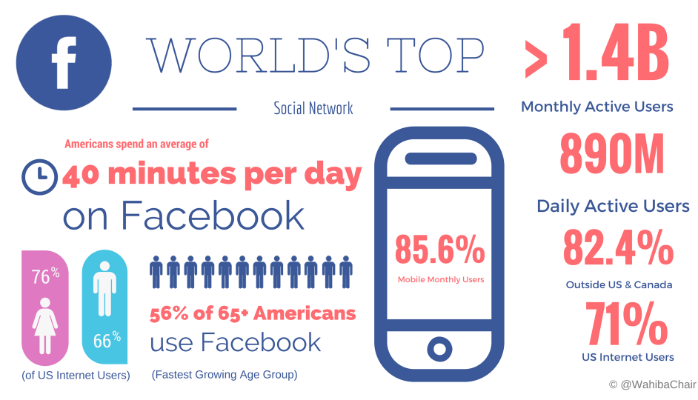
\includegraphics[height=5cm]{../images/SocialMedia2015.png}
\end{center}

A numerical summary describes a certain characteristic of the data in a single value. The notion of a numerical summary is very nice – what is lost in subtlety is gained in simplicity.
For example, in the Australian census data, 1 mean can summarise 21.5 million data points. 
\href{https://www.linkedin.com/pulse/2015-social-media-stats-trends-images-part-1-wahiba-chair-mba}{\beamergotobutton{SocialMediaStats}}
\href{http:\\www.censusdata.abs.gov.au/census_services/getproduct/census/2011/quickstat/0}{\beamergotobutton{AusCensusData}}
\end{frame}

\begin{frame}[fragile]{}

{\bf From the Australian Road Fatalities summaries, what do you learn about the variables?}

{\tiny 
\begin{knitrout}
\definecolor{shadecolor}{rgb}{0.969, 0.969, 0.969}\color{fgcolor}\begin{kframe}
\begin{alltt}
\hlkwd{summary}\hlstd{(data[}\hlnum{1}\hlopt{:}\hlnum{8}\hlstd{])}
\end{alltt}
\begin{verbatim}
##     Crash.ID             State            Date          Day      
##  Min.   :1.202e+12   NSW    :138   17-Apr-16: 10   Min.   : 1.0  
##  1st Qu.:1.202e+12   VIC    :100   20-Feb-16:  9   1st Qu.: 9.0  
##  Median :2.202e+12   QLD    : 76   27-Jan-16:  9   Median :15.0  
##  Mean   :2.973e+12   WA     : 64   5-Mar-16 :  9   Mean   :15.5  
##  3rd Qu.:4.202e+12   SA     : 31   9-Jan-16 :  9   3rd Qu.:22.0  
##  Max.   :8.202e+12   TAS    : 18   16-Feb-16:  8   Max.   :31.0  
##                      (Other): 15   (Other)  :388                 
##       Month          Year           Dayweek        Time    
##  April   :116   Min.   :2016   Friday   :68   13:00  : 10  
##  February:105   1st Qu.:2016   Monday   :50   14:00  : 10  
##  January :106   Median :2016   Saturday :85   21:00  : 10  
##  March   :115   Mean   :2016   Sunday   :56   8:00   : 10  
##                 3rd Qu.:2016   Thursday :58   15:00  :  9  
##                 Max.   :2016   Tuesday  :67   17:00  :  8  
##                                Wednesday:58   (Other):385
\end{verbatim}
\end{kframe}
\end{knitrout}
}
\end{frame}

\begin{frame}[fragile]{}

{\tiny 
\begin{knitrout}
\definecolor{shadecolor}{rgb}{0.969, 0.969, 0.969}\color{fgcolor}\begin{kframe}
\begin{alltt}
\hlkwd{summary}\hlstd{(data[}\hlnum{9}\hlopt{:}\hlnum{18}\hlstd{])}
\end{alltt}
\begin{verbatim}
##       Hour            Min                   Crash.Type  BusInvolvement
##  Min.   : 0.00   Min.   : 0.00   Multiple vehicle:195   No :434       
##  1st Qu.: 8.00   1st Qu.: 0.00   Pedestrian      : 51   Yes:  8       
##  Median :13.00   Median :20.00   Single vehicle  :196                 
##  Mean   :12.52   Mean   :20.84                                        
##  3rd Qu.:17.00   3rd Qu.:35.00                                        
##  Max.   :23.00   Max.   :59.00                                        
##  RigidTruck..Involvement Articulated.Truck..Involvement.   SpeedLimit    
##  No :412                 No :408                         Min.   : -9.00  
##  Yes: 30                 Yes: 34                         1st Qu.: 60.00  
##                                                          Median : 80.00  
##                                                          Mean   : 79.76  
##                                                          3rd Qu.:100.00  
##                                                          Max.   :888.00  
##                                     RoadUser      Gender         Age      
##  Bicyclist (includes pillion passengers): 16   Female:116   Min.   :-9.0  
##  Driver                                 :212   Male  :326   1st Qu.:25.0  
##  Motorcycle pillion passenger           :  4                Median :42.5  
##  Motorcycle rider                       : 89                Mean   :44.6  
##  Passenger                              : 66                3rd Qu.:61.0  
##  Pedestrian                             : 55                Max.   :96.0
\end{verbatim}
\end{kframe}
\end{knitrout}
}
\end{frame}

\begin{frame}[fragile]{}
Note: We use different summaries for different types of variables.  \\

\begin{itemize}
\item {\bf Categorial Data} \\
Categorical data is essentially already summarised by category. We note the most common category or any trend within the categories. \\

\vspace{.5cm}
\item
{\bf Numerical Data} \\
Numerical summaries focus on a feature of interest, like the centre and spread.
\end{itemize}
\end{frame}


\subsection[]{Numerical Data - Notation}
\begin{frame}{Notation for Numerical Summaries}
Given a univariate data set of sample size $n$:

\begin{itemize}
\item
the data is $ \{ x_i \},i=1,2,\ldots,n$   or  $\{ x_{1},x_{2} \ldots, ,x_{n} \}$. 

\vspace{.5cm}
\item the ordered (ascending) data set is $ \{ x_{(i)} \},i=1,2,\ldots,n$ or 
$\{ x_{(1)},x_{(2)},\ldots,x_{(n)} \}$.

\vspace{.5cm}
\item 
the sum of the data is $\sum_{i=1}^{n} x_i = x_1+ x_2+\ldots x_n$.
\end{itemize}
\end{frame}

\begin{frame}[fragile]{}
\begin{alertblock}{Have a try}
Given a data set $\{ 1,4,6,2,3,7\}$, find
\[ \sum_{i=1}^{6} x_{i},  \sum_{i=2}^{5} x_{i}^2, \sum_{i=1}^{6} i x_{i}, \sum_{i=1}^{6} (x_{(i)}-1) \]
\end{alertblock}

\begin{knitrout}
\definecolor{shadecolor}{rgb}{0.969, 0.969, 0.969}\color{fgcolor}\begin{kframe}
\begin{alltt}
\hlcom{#Check your answers}
\hlstd{x}\hlkwb{=}\hlkwd{c}\hlstd{(}\hlnum{1}\hlstd{,}\hlnum{4}\hlstd{,}\hlnum{6}\hlstd{,}\hlnum{2}\hlstd{,}\hlnum{3}\hlstd{,}\hlnum{7}\hlstd{)}
\hlstd{y}\hlkwb{=}\hlkwd{c}\hlstd{(}\hlkwd{sum}\hlstd{(x),} \hlkwd{sum}\hlstd{(x[}\hlnum{2}\hlopt{:}\hlnum{5}\hlstd{]}\hlopt{^}\hlnum{2}\hlstd{),} \hlkwd{sum}\hlstd{(}\hlkwd{c}\hlstd{(}\hlnum{1}\hlopt{:}\hlnum{6}\hlstd{)}\hlopt{*}\hlstd{x),} \hlkwd{sum}\hlstd{(}\hlkwd{sort}\hlstd{(x)}\hlopt{-}\hlnum{1}\hlstd{))}
\hlstd{y}
\end{alltt}
\begin{verbatim}
## [1] 23 65 92 17
\end{verbatim}
\end{kframe}
\end{knitrout}
\href{www.mathsisfun.com/algebra/sigma-notation.html}{\beamergotobutton{More practise here}}
\end{frame}


\subsection[]{Numerical Data - Summaries for Centre}
\begin{frame}[fragile]{Numerical Data - Summaries for Centre}
%[label=SummariesCentre]

There are 2 main measures of the centre (or location) of the data:

\begin{itemize}
\item {\bf Mean} $\bar{x}$ \\
The mean is the average of the data. \\
\[ \bar{x} = \frac{1}{n} \sum_{i=1}^{n} x_{i} \]

\item {\bf Median} $\tilde{x}$ \\
The median is the centre of the data, also called the 50\% percentile or the 2nd quartile. It splits the data into 2 equal groups.  

\begin{itemize}
\item 
If $n$ is odd, the unique median is the middle value:
\[  \tilde{x} = x_{(\frac{n+1}{2})}  \]

\item
If $n$ is even, the median is the average of the 2 middle values (by convention):
\[ \tilde{x} = \frac{x_{(\frac{n}{2})} + x_{(\frac{n}{2} + 1)}}{2} \]
\end{itemize}
\end{itemize}
\end{frame}

\begin{frame}[fragile]{}

\vspace{.5cm}
\begin{alertblock}{Have a try}
For the data: $\{ 1,4,6,2,3,7\}$, show that the mean is 3.83 and the median is 3.5. 
\end{alertblock}

\begin{knitrout}
\definecolor{shadecolor}{rgb}{0.969, 0.969, 0.969}\color{fgcolor}\begin{kframe}
\begin{alltt}
\hlcom{#Check your answers}
\hlstd{x}\hlkwb{=}\hlkwd{c}\hlstd{(}\hlnum{1}\hlstd{,}\hlnum{4}\hlstd{,}\hlnum{6}\hlstd{,}\hlnum{2}\hlstd{,}\hlnum{3}\hlstd{,}\hlnum{7}\hlstd{)}
\hlkwd{mean}\hlstd{(x)}
\end{alltt}
\begin{verbatim}
## [1] 3.833333
\end{verbatim}
\begin{alltt}
\hlkwd{median}\hlstd{(x)}
\end{alltt}
\begin{verbatim}
## [1] 3.5
\end{verbatim}
\end{kframe}
\end{knitrout}

%%%%Extention%%%%
%Note: Data sets which have the same values in the same proportions have the same median (replication principle). For example, the sets $\{ 1,2,3,4 \}$ and $\{ 1,1,1,2,2,2,3,3,3,4,4,4 \}$ have the same median.
\end{frame}


\begin{frame}{Comparing the Mean and Median}
\begin{itemize}
\item 
For symmetric data, we expect $\bar{x} = \tilde{x}$. For left skewed data, we expect $\bar{x} < \tilde{x}$ and for right skewed data, $\bar{x} > \tilde{x}$.
\end{itemize}

\begin{knitrout}
\definecolor{shadecolor}{rgb}{0.969, 0.969, 0.969}\color{fgcolor}
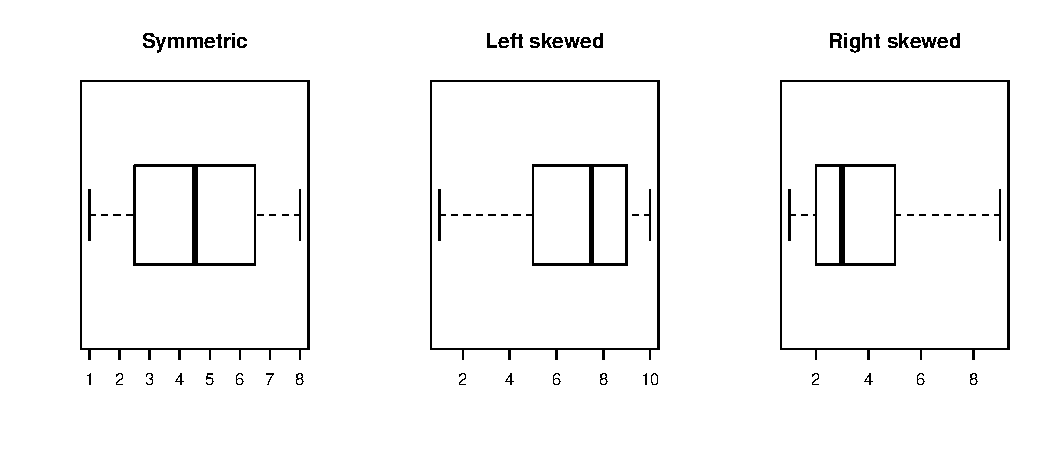
\includegraphics[width=\maxwidth]{figure/unnamed-chunk-7-1} 

\end{knitrout}
\end{frame}


\begin{frame}
\begin{itemize}
\item
Which is ‘optimal’ for describing the centre of the data? 

\vspace{.5cm}
Both have strengths and weaknesses depending on the nature of the data. 
\begin{itemize}
\item Sometimes neither gives a sensible sense of location, for example if the data is bimodal.
\item The median is robust which means it is not affected by some extreme readings. This makes the median preferable for data which is skewed or has many outliers (eg Sydney house prices). 
\item The mean is helpful for data which is basically symmetric which not too many outliers, and for theoretical analysis.
\end{itemize}
\end{itemize}
\end{frame}

\begin{frame}[fragile]{}
\begin{knitrout}
\definecolor{shadecolor}{rgb}{0.969, 0.969, 0.969}\color{fgcolor}\begin{kframe}
\begin{alltt}
\hlstd{Speed} \hlkwb{<-} \hlstd{data}\hlopt{$}\hlstd{SpeedLimit}
\hlkwd{mean}\hlstd{(Speed)}
\end{alltt}
\begin{verbatim}
## [1] 79.76471
\end{verbatim}
\begin{alltt}
\hlkwd{median}\hlstd{(Speed)}
\end{alltt}
\begin{verbatim}
## [1] 80
\end{verbatim}
\begin{alltt}
\hlkwd{par}\hlstd{(}\hlkwc{mfrow} \hlstd{=} \hlkwd{c}\hlstd{(}\hlnum{1}\hlstd{,} \hlnum{2}\hlstd{))}
\hlkwd{boxplot}\hlstd{(Speed,} \hlkwc{horizontal}\hlstd{=T)}
\hlkwd{hist}\hlstd{(Speed)}
\end{alltt}
\end{kframe}
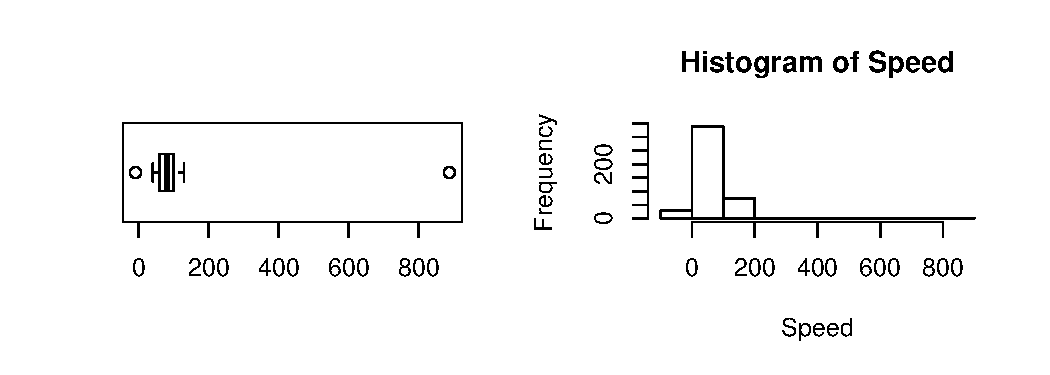
\includegraphics[width=\maxwidth]{figure/unnamed-chunk-8-1} 

\end{knitrout}
\end{frame}


\subsection[]{Numerical Summaries for Spread}
\begin{frame}[fragile]{Numerical Data - Summaries for Spread}
Having summarised the centre of the data, we now want to couple this with a summary of the spread of the data: how far is the data from the centre? The combination of both a numerical centre of centre and spread is a surprisingly helpful snapshot of the data.

\vspace{.5cm}
We can base our summaries for spread on the mean or the quantiles.
\end{frame}

\begin{frame}[fragile]{Spread - based on the Mean (Standard Deviation)}

There are 3 main measures of spread based on the mean:
\begin{itemize}
\item {\bf Mean Absolute Deviation (MAD)}
\[ MAD = \frac{1}{n} \sum_{i=1}^{n} | x_{i} - \bar{x} | \]
This is messy algebraically.

\vspace{.5cm}
\item {\bf Mean Square Error (MSE)}
\[ MSE = \frac{1}{n} \sum_{i=1}^{n} (x_{i} - \bar{x})^2 \]
This requires that we sample $\bar{x}$ from the sample before calculating the MSE: only $n-1$ of the observations are independent of each other.
\end{itemize}
\end{frame}

\begin{frame}[fragile]{}
\begin{itemize}
\item {\bf Standard deviation (SD)}
\[ s= \sqrt{\frac{1}{n-1}  \sum_{i=1}^{n} (x_{i} - \bar{x})^2 } \]

This is called the definition formula: it represents the average of the squared deviations from the mean $\{ (x_{i} - \bar{x}) \}$. We need squared deviations as $\sum_{i=1}^{n} (x_{i} - \bar{x}) = 0$.

\vspace{.5cm}
The calculation formula is
\[ s= \sqrt{\frac{1}{n-1} \big[ \sum_{i=1}^{n} x_{i}^2 - \frac{1}{n} (\sum_{i=1}^{n} x_{i})^2 \big] }
= \sqrt{ \frac{1}{n-1} \big[ \sum_{i=1}^{n} x_{i}^2 - n \bar{x}^2} \big]
\]

\vspace{.5cm}
$s^2 = \frac{1}{n-1} \sum_{i=1}^{n-1} (x_{i} - \bar{x})^2$ is called the variance. 
\end{itemize}
\end{frame}

\begin{frame}[fragile]{Using the Standard Deviation}
Note that $s$ has the same units as $\bar{x}$, so we can couple $(\bar{x}, s)$ as a summary of centre and spread.

\vspace{.5cm}
\begin{block}{Calculating Standard Deviation}
Given $\{ 1,4,6,2,3,7\}$ with $\bar{x}=23/6$, what is the standard deviation? \\

Definition formula: $s= \sqrt{ \frac{1}{5} [ (1-23/6)^2 + (4-23/6)^2 + \ldots (7-23/6)^2 ]} \approx 2.32 $ \\

Calculation formula: $s = \sqrt{ \frac{1}{5} [ 1^2 + 4^2 + 6^2 + 2^2 + 3^2 + 7^2 - 6(23/6)^2] }  \approx 2.32 $

\end{block}

\begin{knitrout}
\definecolor{shadecolor}{rgb}{0.969, 0.969, 0.969}\color{fgcolor}\begin{kframe}
\begin{alltt}
\hlkwd{sd}\hlstd{(x)}
\end{alltt}
\begin{verbatim}
## [1] 2.316607
\end{verbatim}
\end{kframe}
\end{knitrout}
\end{frame}
 
 
 
\begin{frame}[fragile]{}
\begin{knitrout}
\definecolor{shadecolor}{rgb}{0.969, 0.969, 0.969}\color{fgcolor}\begin{kframe}
\begin{alltt}
\hlstd{Speed} \hlkwb{<-} \hlstd{data}\hlopt{$}\hlstd{SpeedLimit}
\hlkwd{mean}\hlstd{(Speed)}
\end{alltt}
\begin{verbatim}
## [1] 79.76471
\end{verbatim}
\begin{alltt}
\hlkwd{median}\hlstd{(Speed)}
\end{alltt}
\begin{verbatim}
## [1] 80
\end{verbatim}
\begin{alltt}
\hlkwd{sd}\hlstd{(Speed)}
\end{alltt}
\begin{verbatim}
## [1] 49.54275
\end{verbatim}
\begin{alltt}
\hlstd{iqr}\hlkwb{=}\hlkwd{fivenum}\hlstd{(Speed)[}\hlnum{4}\hlstd{]}\hlopt{-}\hlkwd{fivenum}\hlstd{(Speed)[}\hlnum{2}\hlstd{]}
\hlstd{iqr}
\end{alltt}
\begin{verbatim}
## [1] 40
\end{verbatim}
\end{kframe}
\end{knitrout}
\end{frame}

\begin{frame}[fragile]{}
\begin{knitrout}
\definecolor{shadecolor}{rgb}{0.969, 0.969, 0.969}\color{fgcolor}\begin{kframe}
\begin{alltt}
\hlkwd{fivenum}\hlstd{(Speed)}
\end{alltt}
\begin{verbatim}
## [1]  -9  60  80 100 888
\end{verbatim}
\begin{alltt}
\hlkwd{boxplot}\hlstd{(Speed,} \hlkwc{horizontal}\hlstd{=T)}
\end{alltt}
\end{kframe}
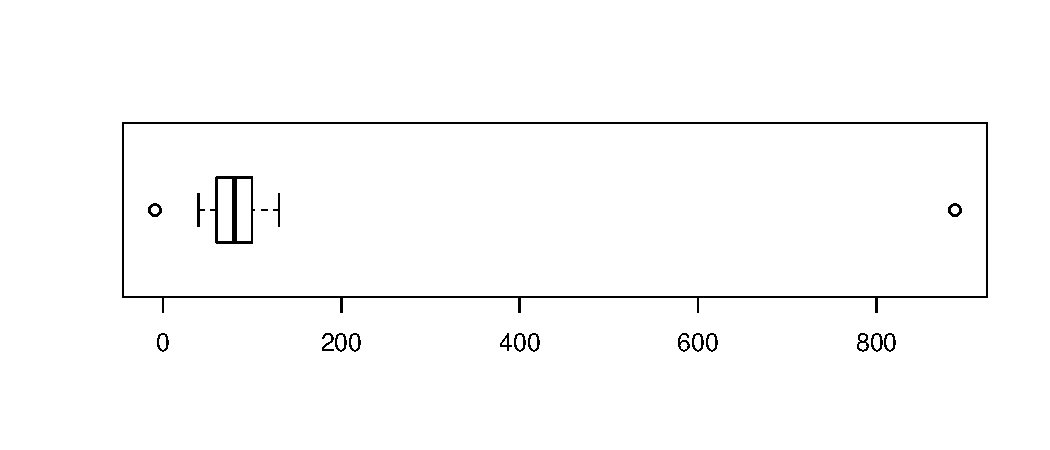
\includegraphics[width=\maxwidth]{figure/unnamed-chunk-11-1} 

\end{knitrout}
\end{frame}
 
 
 
 
\begin{frame}[fragile,label=Quartiles]{Spread - based on the Quartiles (IQR)}
The quartiles are a set of 3 values $\{ Q_{1}, Q_{2} = \tilde{x}, Q_{3} \}$ that roughly split the data into quarters.

\vspace{.5cm}
There is no universal way to define quartiles.  
We use the following convention: we divide the data into 2 sets at the median (including the median for an odd sized data set), and then find the median of each half set of data.

\vspace{.5cm}
Once we have found $Q_{1}$, we can find $Q_{3}$ by symmetry, by counting back from the end of sorted data set.
\end{frame}


\begin{frame}[fragile]{}
\begin{block}{Calculating the Quartiles (even sized sample)}
Given $\{ 1,4,6,2,3,7\}$, the sorted data is $\{ 1,2,3,4,6,7 \}$ and the median $Q_{2} = 3.5$ splits the data into $\{ 1,2,3 \}$ and $\{ 4,6,7 \}$, hence $Q_{1} = 2$ and $Q_{3} = 6$.
\end{block}

\begin{knitrout}
\definecolor{shadecolor}{rgb}{0.969, 0.969, 0.969}\color{fgcolor}\begin{kframe}
\begin{alltt}
\hlcom{# Finds min, Q1, Q2, Q3, max}
\hlkwd{fivenum}\hlstd{(x)}
\end{alltt}
\begin{verbatim}
## [1] 1.0 2.0 3.5 6.0 7.0
\end{verbatim}
\end{kframe}
\end{knitrout}
\end{frame}

\begin{frame}[fragile]{}
\begin{block}{Calculating the Quartiles (even sized sample)}
Given $\{ 1,4,6,2,3,7\}$, the sorted data is $\{ 1,2,3,4,6,7 \}$ and the median $Q_{2} = 3.5$ splits the data into $\{ 1,2,3 \}$ and $\{ 4,6,7 \}$, hence $Q_{1} = 2$ and $Q_{3} = 6$.
\end{block}

\begin{knitrout}
\definecolor{shadecolor}{rgb}{0.969, 0.969, 0.969}\color{fgcolor}\begin{kframe}
\begin{alltt}
\hlcom{# Finds min, Q1, Q2, Q3, max}
\hlkwd{fivenum}\hlstd{(x)}
\end{alltt}
\begin{verbatim}
## [1] 1.0 2.0 3.5 6.0 7.0
\end{verbatim}
\end{kframe}
\end{knitrout}
\end{frame}

\begin{frame}[fragile]{}
\begin{block}{Calculating the Quartiles (odd sized sample)}
Given $\{ 1,4,6,2,3,7,8\}$, the sorted data is $\{ 1,2,3,4,6,7,8 \}$ and the median $Q_{2} = 4$ splits the data into $\{ 1,2,3,4 \}$ and $\{ 4,6,7,8 \}$, hence $Q_{1} = 2.5$ and $Q_{3} = 6.5$.
\end{block}

\begin{knitrout}
\definecolor{shadecolor}{rgb}{0.969, 0.969, 0.969}\color{fgcolor}\begin{kframe}
\begin{alltt}
\hlstd{x2}\hlkwb{=}\hlkwd{c}\hlstd{(}\hlnum{1}\hlstd{,}\hlnum{4}\hlstd{,}\hlnum{6}\hlstd{,}\hlnum{2}\hlstd{,}\hlnum{3}\hlstd{,}\hlnum{7}\hlstd{,}\hlnum{8}\hlstd{)}
\hlkwd{fivenum}\hlstd{(x2)}
\end{alltt}
\begin{verbatim}
## [1] 1.0 2.5 4.0 6.5 8.0
\end{verbatim}
\end{kframe}
\end{knitrout}
\end{frame}


\begin{frame}[fragile]{Interquartile Range (IQR)}
The full range of the data is $x_{(n)} - x_{(1)}$, but this ignores $n-2$ data points.

\vspace{.5cm}
The Interquartile Range is defined as
\[ IQR = Q_{3} -Q_{1} \]
and represents the range of the middle 50\% of the data. 

\vspace{.5cm}
We couple $(\tilde{x}, IQR)$ as a summary of centre and spread.
\begin{knitrout}
\definecolor{shadecolor}{rgb}{0.969, 0.969, 0.969}\color{fgcolor}\begin{kframe}
\begin{alltt}
\hlkwd{fivenum}\hlstd{(x)[}\hlnum{4}\hlstd{]}\hlopt{-}\hlkwd{fivenum}\hlstd{(x)[}\hlnum{2}\hlstd{]}   \hlcom{# Don't use iqr()}
\end{alltt}
\begin{verbatim}
## [1] 4
\end{verbatim}
\end{kframe}
\end{knitrout}
\end{frame}

\begin{frame}[fragile]{The Five Number Summary}
The five number summary is a neat way to summarise the data
\[ ( x_{(1)}, Q_{1}, Q_{2}, Q_{3}, x_{(n)} ) \]
and is essentially drawn by the boxplot.

\begin{knitrout}
\definecolor{shadecolor}{rgb}{0.969, 0.969, 0.969}\color{fgcolor}\begin{kframe}
\begin{alltt}
\hlkwd{fivenum}\hlstd{(x)}
\end{alltt}
\begin{verbatim}
## [1] 1.0 2.0 3.5 6.0 7.0
\end{verbatim}
\begin{alltt}
\hlkwd{boxplot}\hlstd{(x,} \hlkwc{horizontal}\hlstd{=T,} \hlkwc{col}\hlstd{=}\hlstr{"purple"}\hlstd{)}
\end{alltt}
\end{kframe}
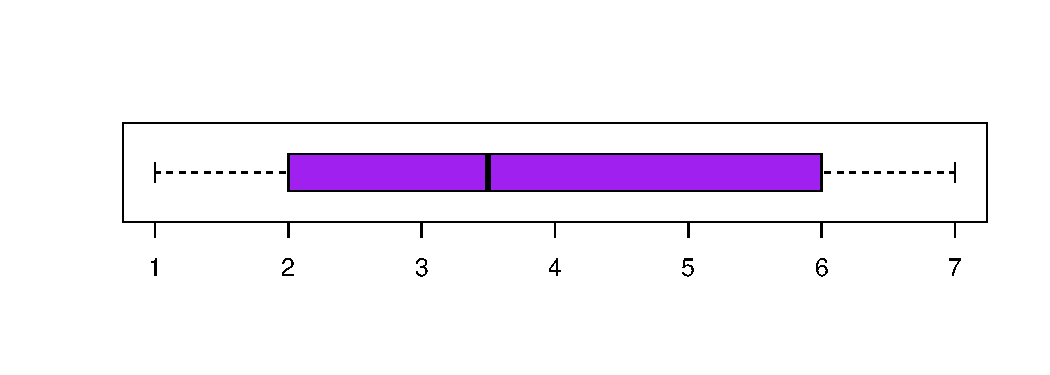
\includegraphics[width=\maxwidth]{figure/unnamed-chunk-16-1} 

\end{knitrout}
\end{frame}

\begin{frame}[fragile]{Comparing the SD and the IQR}
Like the mean and median, the IQR is robust and so preferable for data which is skewed or has many outliers. However, the standard deviation is good for theoretical analysis.

\vspace{.5cm}
\begin{block}{Comparing the SD and the IQR}
Given $\{ 1,4,6,2,3,7,100\}$, what is the sd and IQR?
\end{block}

\begin{knitrout}
\definecolor{shadecolor}{rgb}{0.969, 0.969, 0.969}\color{fgcolor}\begin{kframe}
\begin{alltt}
\hlstd{x1}\hlkwb{=}\hlkwd{c}\hlstd{(}\hlnum{1}\hlstd{,}\hlnum{4}\hlstd{,}\hlnum{6}\hlstd{,}\hlnum{2}\hlstd{,}\hlnum{3}\hlstd{,}\hlnum{7}\hlstd{,}\hlnum{100}\hlstd{)}
\hlkwd{sd}\hlstd{(x1)}
\end{alltt}
\begin{verbatim}
## [1] 36.40905
\end{verbatim}
\begin{alltt}
\hlkwd{fivenum}\hlstd{(x1)[}\hlnum{4}\hlstd{]} \hlopt{-} \hlkwd{fivenum}\hlstd{(x1)[}\hlnum{2}\hlstd{]}
\end{alltt}
\begin{verbatim}
## [1] 4
\end{verbatim}
\end{kframe}
\end{knitrout}
\end{frame}

\subsection[]{Outliers}
\begin{frame}[fragile]{Identifying Outliers}
Outliers are `unusual values' that do not fit the model. They can either indicate interesting values that need futher investigation or a transformation of the model, or they can indicate a possible mistake in your data.

\vspace{.5cm}
There are 2 main ways to identify outliers:
\begin{itemize}
\item {\bf The IQR method (Tukey)} \\
As outlined in the boxplot, we calculate the lower and upper thresholds
\[ LT = Q_{1} - 1.5 IQR  \mbox{  and   }  UT = Q_{3} + 1.5 IQR  \]
Any data point lying outside these thresholds is deemed an outlier. \\
Disadvantages:  No outliers detected for $n \leq 4$ and for large samples wrongly identifies outliers.
\end{itemize}
\end{frame}

\begin{frame}[fragile]{Identifying Outliers}
\begin{itemize}
\item {\bf (Extension: The 3-$\sigma$ method)} \\
Any data point lying more than 3 standard deviations away from the mean is deemed to be an outlier. \\
\[ x_{i} \mbox{ is an outlier iff } |x_{i} - \bar{x}| > 3 \sigma  \]
Disadvantages:  No outliers detected for $n \leq 7$ and for large samples wrongly identifies outliers. \\

\vspace{.5cm}
Note: The 3-sigma edit rule is popular in economics, but it should be avoided in practice due to the following inflexibility, which will make more sense after Part2 of the course. 
\end{itemize}
\end{frame}

\begin{frame}[fragile]{}
The 3-$\sigma$ rule assumes that the underlying distribution is the Normal, and is based on both the sample mean and standard deviation. Problems can occur when either:

\vspace{.5cm}
1) The data is sufficiently skewed. In this case, the mean is no longer a `good' measure of central tendency, and defining outliers as points outside of some symmetric neighbourhood of the mean is not appropriate. The risk is that the `outliers' are detected near the mode rather than the longer tail. Tukey's five number approach is less likely to suffer from this.  
\end{frame}

\begin{frame}[fragile]{}
2) The underlying population has heavy tails. The principle behind the 3-$\sigma$ rule is that $P(  |x_{i} - \bar{x}| > 3 \sigma)$ occurs with small probability, for example when the population is Normal this probability is 0.0027. 

\begin{knitrout}
\definecolor{shadecolor}{rgb}{0.969, 0.969, 0.969}\color{fgcolor}\begin{kframe}
\begin{alltt}
\hlnum{2}\hlopt{*}\hlstd{(}\hlnum{1}\hlopt{-}\hlkwd{pnorm}\hlstd{(}\hlnum{3}\hlstd{))}
\end{alltt}
\begin{verbatim}
## [1] 0.002699796
\end{verbatim}
\end{kframe}
\end{knitrout}

\vspace{.5cm}
If there are heavy tails then this probability can be substantially larger. For example, the probability is 0.029 when the population is $t_{3}$, or 0.10 when the population is $t_{1}$. In the latter case 10\% of the observations will be deemed `outliers'!

%{\tiny 
%<<>>=
%2*(1-pt(3*sqrt(3),3))
%2*(1-pt(3*sqrt(2),1))
%@
%}

\end{frame}


\begin{frame}[fragile]{}
\begin{block}{Detecting Outlier in Data with Mistake}
Suppose we made a mistake in the data entry with heights:
1.68 1.58 1.64 1.73 1.60 1.62 1.78 1.69 1.80 1.74 1.71 1.59 1.63 1.77 1.70 1.77 1.63 1.62 1.80 1.70 1.60 1.77 1.79 1.65 1.66 1.60 1.71 {\bf 178}
\end{block}

IQR method
\begin{knitrout}
\definecolor{shadecolor}{rgb}{0.969, 0.969, 0.969}\color{fgcolor}\begin{kframe}
\begin{alltt}
\hlcom{## Usyd <- read.csv("USyd.csv")}
\hlstd{heights1}\hlkwb{=}\hlkwd{c}\hlstd{(Usyd}\hlopt{$}\hlstd{Heights[}\hlnum{1}\hlopt{:}\hlnum{27}\hlstd{],}\hlnum{178}\hlstd{)}
\hlstd{iqr}\hlkwb{=}\hlkwd{fivenum}\hlstd{(heights1)[}\hlnum{4}\hlstd{]}\hlopt{-}\hlkwd{fivenum}\hlstd{(heights1)[}\hlnum{2}\hlstd{]}
\hlstd{lt}\hlkwb{=}\hlkwd{fivenum}\hlstd{(heights1)[}\hlnum{2}\hlstd{]}\hlopt{-}\hlnum{1.5}\hlopt{*}\hlstd{iqr}
\hlstd{ut}\hlkwb{=}\hlkwd{fivenum}\hlstd{(heights1)[}\hlnum{4}\hlstd{]}\hlopt{+}\hlnum{1.5}\hlopt{*}\hlstd{iqr}
\hlstd{heights1[(heights1}\hlopt{<}\hlstd{lt)} \hlopt{|} \hlstd{(heights1} \hlopt{>} \hlstd{ut)]}   \hlcom{# | = 'or'}
\end{alltt}
\begin{verbatim}
## [1] 178
\end{verbatim}
\end{kframe}
\end{knitrout}
\end{frame}

\begin{frame}[fragile]{}
3-$\sigma$ method
\begin{knitrout}
\definecolor{shadecolor}{rgb}{0.969, 0.969, 0.969}\color{fgcolor}\begin{kframe}
\begin{alltt}
\hlnum{3}\hlopt{*}\hlkwd{sd}\hlstd{(heights1)}
\end{alltt}
\begin{verbatim}
## [1] 99.95986
\end{verbatim}
\begin{alltt}
\hlstd{heights1[}\hlkwd{abs}\hlstd{(heights1}\hlopt{-}\hlkwd{mean}\hlstd{(heights1))}\hlopt{>}\hlnum{3}\hlopt{*}\hlkwd{sd}\hlstd{(heights1)]}
\end{alltt}
\begin{verbatim}
## [1] 178
\end{verbatim}
\end{kframe}
\end{knitrout}
\end{frame}


\begin{frame}[fragile]{Dealing with Outliers by Transformation}
Sometimes an outlier indicates that a better model is needed.
\begin{knitrout}
\definecolor{shadecolor}{rgb}{0.969, 0.969, 0.969}\color{fgcolor}\begin{kframe}
\begin{alltt}
\hlstd{w}\hlkwb{=}\hlkwd{c}\hlstd{(}\hlnum{1}\hlstd{,}\hlnum{2}\hlstd{,}\hlnum{3}\hlstd{,}\hlnum{4}\hlstd{,}\hlnum{10}\hlstd{,}\hlnum{30}\hlstd{,}\hlnum{60}\hlstd{,}\hlnum{120}\hlstd{,}\hlnum{180}\hlstd{,}\hlnum{300}\hlstd{)}
\hlstd{w1}\hlkwb{=}\hlkwd{log}\hlstd{(w,}\hlnum{10}\hlstd{)}
\hlkwd{par}\hlstd{(}\hlkwc{mfrow} \hlstd{=} \hlkwd{c}\hlstd{(}\hlnum{1}\hlstd{,} \hlnum{2}\hlstd{))}
\hlkwd{boxplot}\hlstd{(w,} \hlkwc{main} \hlstd{=}\hlstr{"Data"}\hlstd{)}
\hlkwd{boxplot}\hlstd{(w1,} \hlkwc{main}\hlstd{=}\hlstr{"Log of Data"}\hlstd{)}
\end{alltt}
\end{kframe}
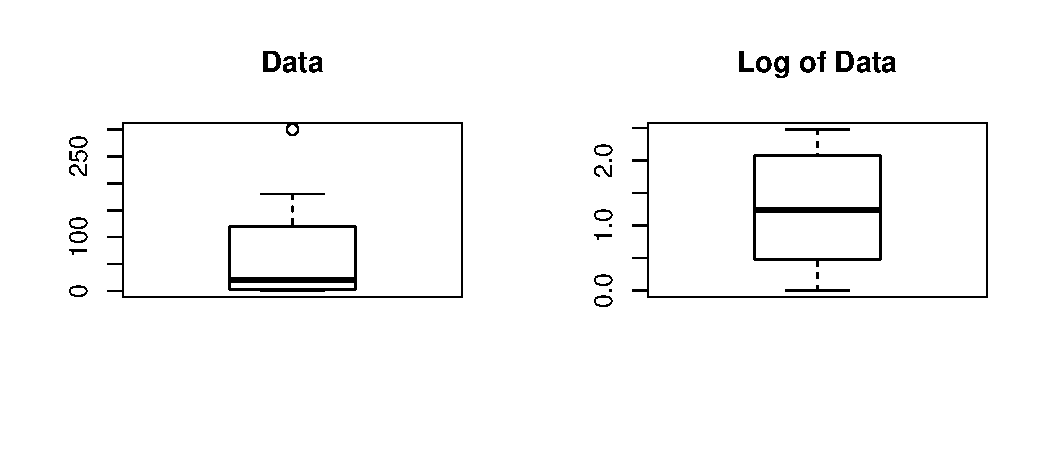
\includegraphics[width=\maxwidth]{figure/unnamed-chunk-21-1} 

\end{knitrout}
\end{frame}
\end{document}
